\section[Groundwork]{Groundwork}
\sectionframe{02}{Groundwork}{Which methods does the paper build on?}{\faBookOpen}

% ----------------------------------------------------- three ways to generate
\begin{frame}[source={Kingma and Welling (2013), arXiv:1312.6114 · Goodfellow et al.\ (2014), NeurIPS · Ramesh et al.\ (2021), ICML · Ho et al.\ (2020), NeurIPS · Rombach et al.\ (2022), CVPR}]
  {Three ways to generate an image}
  \begin{tikzpicture}[x=1mm,y=1mm]
    \useasboundingbox (0,0) rectangle (144,-54);
    \foreach \i/\c/\h in {0/udsblue/In one pass,1/udsgreymid/Token by token,2/udsblue/Step by step from noise} {
      \pgfmathsetmacro\cx{\i*49}
      \fill[\c!8] (\cx,-5.4) rectangle ++(46,-41.6);
      \cardhead{\cx}{0}{46}{\c}{\h}
    }
    % in one pass: a code, decoded into the whole image
    \filldraw[fill=udsblue,draw=udsblue] (6,-12.3) rectangle (10.4,-19.7);
    \node[text=white,font=\small\itshape,inner sep=0pt] at (8.2,-16) {z};
    \draw[flow] (11,-16) -- (14.2,-16);
    \filldraw[fill=bluetint,draw=udsblue,line width=0.5pt] (15,-12.5) -- (25.4,-9) -- (25.4,-23) -- (15,-19.5) -- cycle;
    \node[label text,rotate=90] at (20.2,-16) {decoder};
    \draw[flow] (26,-16) -- (29.2,-16);
    \node[anchor=north west,inner sep=0pt] at (30,-9.5) {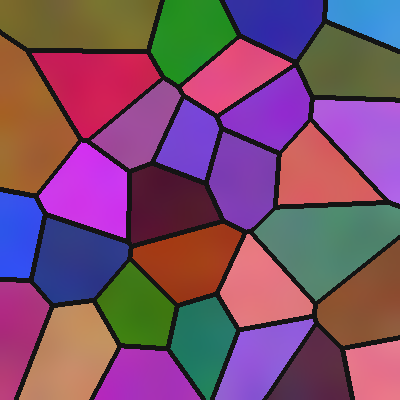
\includegraphics[width=13mm]{assets/drawn/grain-map-new}};
    % token by token: tiles written in reading order, the next one outlined
    \node[anchor=north west,inner sep=0pt] at (65,-9) {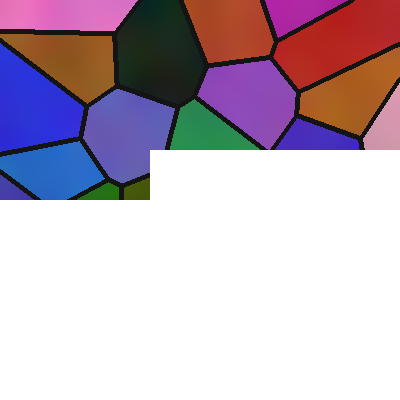
\includegraphics[width=14mm]{assets/drawn/tokens-partial}};
    \begin{scope}[shift={(65,-23)}]
      \draw[udsgreylight,line width=0.3pt] (0,0) grid[step=1.75] (14,14);
      \draw[udsred,line width=0.8pt] (5.25,7) rectangle (7,8.75);
    \end{scope}
    % step by step from noise: the whole image refined at every step
    \foreach \t/\x in {1000/100.5,150/116,0/131.5}
      \node[anchor=north west,inner sep=0pt] at (\x,-10.5) {\includegraphics[width=11mm]{assets/drawn/diffusion-t\t}};
    \draw[flow,draw=udsblue] (112,-16) -- (115.4,-16);
    \draw[flow,draw=udsblue] (127.5,-16) -- (130.9,-16);
    % what each does, examples, and how the image is built
    \foreach \i/\a/\e/\b in {0/{a decoder turns a code into an image}/{VAE (2013), GAN (2014)}/{whole image at once},
        1/{a network predicts each tile from the tiles before it}/{DALL-E 1 (2021); language models write text
          this way}/{no going back to refine},
        2/{a network removes a little noise at each step}/{DDPM (2020), Stable Diffusion (2022), DALL-E 2
          (2022)}/{refines the whole image}} {
      \node[card text,text width=42mm] at ({\i*49+2},-26.6) {\a};
      \node[card text,text width=42mm,font=\scriptsize,text=udsgrey] at ({\i*49+2},-35) {\e};
      \node[card text,text width=42mm,font=\footnotesize\bfseries] at ({\i*49+2},-42.4) {\b};}
    \node[anchor=north west,small label,text=udsred] at (0,-49.4)
      {Liao et al.\ join the first and the third: the VAE output guides the diffusion steps};
  \end{tikzpicture}
  \note{\textbf{4:20--5:20}\par
    Generative models differ in how they build an image.\par
    In one pass: a decoder turns a short code into the whole image at once; VAEs and GANs work this
      way.\par
    Token by token: a network predicts each piece of the image from the pieces before it, as language
      models write text word by word; DALL-E 1 (Ramesh and colleagues, 2021) wrote 32 by 32 such tokens,
      which a discrete VAE then decoded into the image.\par
    Such a model starts from scratch and works in a fixed order, so it cannot go back and refine what it
      has written.\par
    Step by step from noise: a diffusion model starts from noise and refines the whole image at every
      step; Stable Diffusion and DALL-E 2 and 3 work this way, and diffusion leads image generation
      today.\par
    The paper joins the first and the third: a VAE generates in one pass, and its output guides the
      diffusion steps.}
\end{frame}

% ------------------------------------------------------------------ VAE
\begin{frame}[source={Kingma and Welling (2013), arXiv:1312.6114}]{Variational Autoencoder (VAE)}
  \begin{tikzpicture}[x=1mm,y=1mm]
    \useasboundingbox (0,0) rectangle (144,-54);
    \tikzset{part/.style={fill=bluetint,draw=udsblue,line width=0.5pt}}
    % encode, sample, decode; the row's centre line is y = -11.5
    \node[anchor=north west,inner sep=0pt] at (0,-5.5) {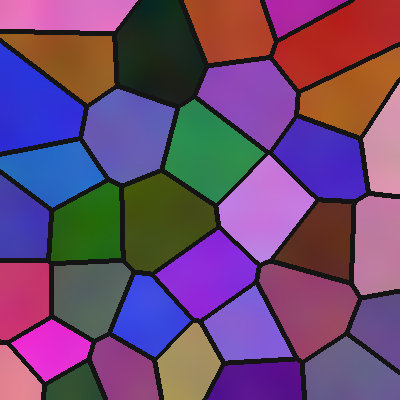
\includegraphics[width=12mm]{assets/drawn/grain-map}};
    \node[anchor=north,small label,text=udsdark] at (6,-18.4) {patch};
    \draw[flow] (12.6,-11.5) -- (16.6,-11.5);
    \filldraw[part] (17.4,-4) -- (27.8,-7.5) -- (27.8,-15.5) -- (17.4,-19) -- cycle;
    \node[label text,rotate=90] at (22.6,-11.5) {encoder};
    \draw[flow] (28.4,-11.5) -- (31.4,-11.5);
    \filldraw[fill=bluetint,draw=udsblue,line width=0.5pt] (32,-6.8) rectangle (36,-11.1);
    \filldraw[fill=darktint,draw=udsdark,line width=0.5pt] (32,-11.9) rectangle (36,-16.2);
    \node[font=\scriptsize,inner sep=0pt,text=udsdark] at (34,-8.95) {$\mu$};
    \node[font=\scriptsize,inner sep=0pt,text=udsdark] at (34,-14.05) {$\sigma$};
    \node[anchor=north,small label,text=udsdark,align=center] at (34,-18.4) {mean,\\ spread};
    \draw[flow] (36.6,-11.5) -- (39.6,-11.5);
    % sample: a normal curve with one drawn value
    \draw[udsgreymid,line width=0.4pt] (40.4,-14.5) -- (49.6,-14.5);
    \draw[udsblue,line width=0.7pt] plot[domain=-2.6:2.6,samples=41] ({45+\x*1.75},{-14.5+6.5*exp(-((\x)^2)/2)});
    \node[circle,fill=udsred,inner sep=0pt,minimum size=1.5mm] at (46.6,-14.5) {};
    \node[anchor=north,small label,text=udsdark] at (45,-18.4) {sample $z$};
    \draw[flow] (50.2,-11.5) -- (53.2,-11.5);
    \filldraw[part] (54,-7.5) -- (64.4,-4) -- (64.4,-19) -- (54,-15.5) -- cycle;
    \node[label text,rotate=90] at (59.2,-11.5) {decoder};
    \draw[flow] (65,-11.5) -- (69,-11.5);
    \node[anchor=north west,inner sep=0pt] at (69.6,-5.5) {
\includegraphics[width=12mm]{assets/drawn/grain-map-blurred}};
    \node[anchor=north,small label,text=udsdark] at (75.6,-18.4) {reconstruction};
    % the loss, each term labelled
    \node[font=\large,text=udsdark,inner sep=0pt] at (4,-32) {$L\;=$};
    \node[font=\large,text=udsdark,inner sep=0pt] (rec) at (21,-32) {$L_{\mathrm{rec}}$};
    \node[font=\large,text=udsdark,inner sep=0pt] at (41,-32) {$+$};
    \node[font=\large,text=udsblue,inner sep=0pt] (kl) at (62,-32) {$L_{\mathrm{KL}}$};
    \node[anchor=north,label text,align=center,text width=28mm] at (21,-36.4) {output close\\ to the input};
    \node[anchor=north,label text,align=center,text width=28mm,text=udsblue] at (62,-36.4)
      {codes close to\\ a standard normal};
    % the latent space: each patch's code is a small cloud, and the clouds overlap
    \draw[udsgreymid,line width=0.5pt] (92,0) rectangle (144,-44);
    \node[anchor=north west,small label] at (93.4,-1.4) {latent space, 2 of 128 directions};
    \foreach \x/\y in {104/-24,110/-18,111/-29,117/-23,103/-33,118/-33,124/-27,109/-38,98/-28}
      {\fill[udsblue,fill opacity=0.14] (\x,\y) circle (4.4); \fill[udsblue] (\x,\y) circle (0.55);}
    \node[text=udsred,font=\footnotesize,inner sep=0pt] (new) at (114.2,-24.4) {\faStar};
    \node[anchor=north west,inner sep=0pt] (np) at (129.4,-9.4) {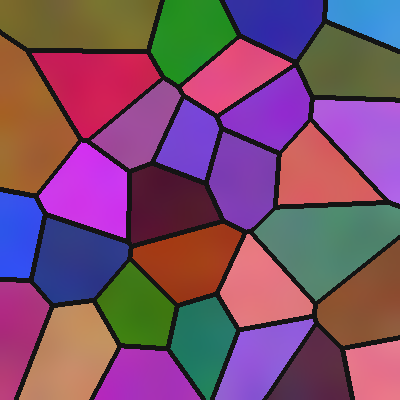
\includegraphics[width=11mm]{assets/drawn/grain-map-new}};
    \draw[udsred,line width=0.7pt,-{Stealth[length=1.6mm,width=1.2mm]}] (new.north east) to[out=40,in=200] (np.west);
    \node[anchor=north,small label,text=udsred,align=center] at (134.9,-21.2) {new code,\\ new patch};
  \end{tikzpicture}
  \note{\textbf{5:20--6:40}\par
    An autoencoder is a network trained to copy its input through a bottleneck: an encoder compresses the
      image into a few numbers, the latent code, and a decoder rebuilds the image from them.\par
    The variational autoencoder, from Kingma and Welling in 2013, makes the code probabilistic: the
      encoder gives a mean and a spread for each number, and the decoder sees a value drawn from that
      range.\par
    A Kullback--Leibler (KL) term pulls every code towards a standard normal distribution, so the codes
      of different images overlap and the space has no gaps.\par
    That makes a VAE generative: a code drawn from this space decodes to a plausible image, and moving
      through the space changes the image smoothly.\par
    Trained with a pixel loss, a VAE returns blurry images, the average of the plausible answers: the
      failure of slide 3.\par
    In this paper each patch gets a code of 128 numbers.}
\end{frame}

% ----------------------------------------------- reconstruct, generate, extrapolate
\begin{frame}{Reconstruct, generate, extrapolate}
  \begin{tikzpicture}[x=1mm,y=1mm]
    \useasboundingbox (0,0) rectangle (144,-54);
    \tikzset{code/.style={circle,fill=udsgreymid,inner sep=0pt,minimum size=1.2mm}}
    \foreach \i/\c/\h in {0/udsdark/Reconstruct,1/udsblue/Generate,2/udsred/Extrapolate} {
      \pgfmathsetmacro\cx{\i*49}
      \fill[\c!8] (\cx,-5.4) rectangle ++(46,-41.6);
      \cardhead{\cx}{0}{46}{\c}{\h}
      % the training codes, the same cloud in every card
      \begin{scope}[shift={(\cx,0)}]
        \filldraw[fill=white,draw=udsgreylight,line width=0.5pt] (21,-16.5) ellipse (8.6 and 5.6);
        \foreach \x/\y in {16/-15,18.6/-19,20.4/-13.6,22.6/-17.4,24.8/-14.6,26.2/-18.4,15.4/-17.8,19.4/-16.2}
          \node[code] at (\x,\y) {};
      \end{scope}
    }
    % reconstruct: a training patch, encoded and decoded
    \node[anchor=north west,inner sep=0pt] (in) at (1.4,-11.5) {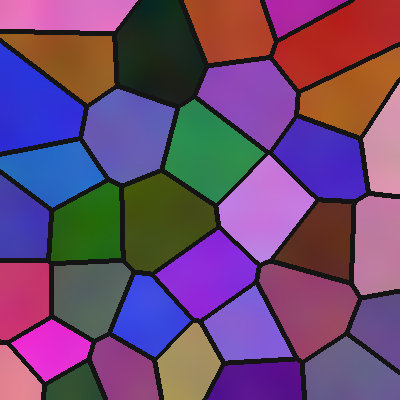
\includegraphics[width=10mm]{assets/drawn/grain-map}};
    \node[circle,draw=udsdark,line width=0.7pt,inner sep=0pt,minimum size=2.6mm] (c0) at (22.6,-17.4) {};
    \draw[flow,line width=0.5pt] (in.east) to[out=0,in=180] (c0.west);
    \node[anchor=north west,inner sep=0pt] (out0) at (34.6,-11.5) {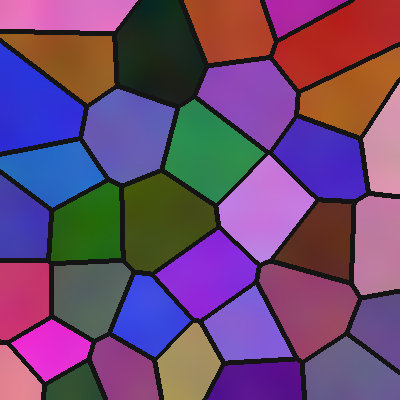
\includegraphics[width=10mm]{assets/drawn/grain-map}};
    \draw[flow,line width=0.5pt] (c0.east) to[out=0,in=180] (out0.west);
    % generate: a new code among the training codes
    \node[circle,fill=udsblue,inner sep=0pt,minimum size=2mm] (c1) at (49+23.4,-15.6) {};
    \node[anchor=north west,inner sep=0pt] (out1) at (49+34.6,-11.5) {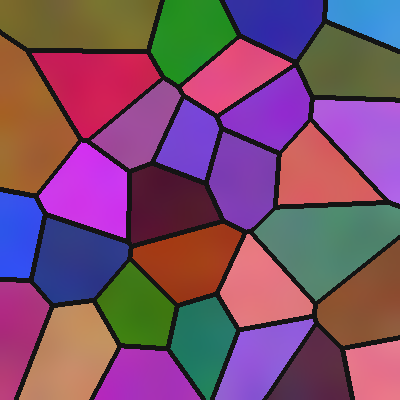
\includegraphics[width=10mm]{assets/drawn/grain-map-new}};
    \draw[flow,draw=udsblue,line width=0.5pt] (c1.east) to[out=0,in=180] (out1.west);
    % extrapolate: a code away from every training code
    \node[text=udsred,font=\footnotesize,inner sep=0pt] (c2) at (98+31.4,-25.4) {\faStar};
    \node[anchor=north west,inner sep=0pt] (out2) at (98+34.6,-11.5) {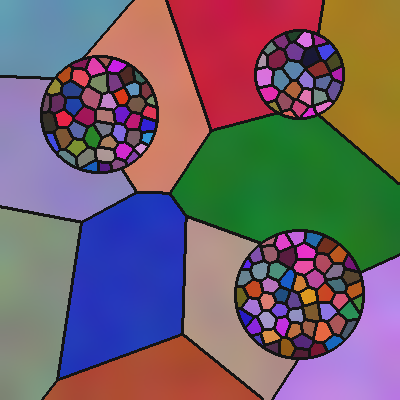
\includegraphics[width=10mm]{assets/drawn/grain-map-bimodal}};
    \node[circle,fill=white,draw=udsred,line width=0.6pt,inner sep=0pt,minimum size=4.2mm,font=\scriptsize\bfseries,
      text=udsred] at ([xshift=-1mm,yshift=1mm]out2.north east) {?};
    \draw[flow,draw=udsred,line width=0.5pt] (c2.east) to[out=0,in=-90] (out2.south);
    % what each is, and what can check it
    \foreach \i/\a/\b in {0/{a training patch, encoded and decoded}/{compare with its input},
        1/{a new code among the training codes}/{compare with held-out data},
        2/{a code away from all training codes}/{only an experiment can tell}} {
      \node[anchor=north west,card text,text width=42mm] at ({\i*49+2},-29.4) {\a};
      \node[anchor=north west,card text,text width=42mm,font=\footnotesize\bfseries] at ({\i*49+2},-41.4) {\b};}
  \end{tikzpicture}
  \note{\textbf{6:40--7:40}\par
    A trained generative model can do three different things, and each needs a different check.\par
    Reconstruct: encode a training patch and decode it again; the result can be compared with its own
      input, pixel by pixel or by its statistics.\par
    Generate: decode a new code from among the training codes; the result has no original, so it is
      compared with the statistics of held-out data and checked for near-copies of training patches.\par
    Extrapolate: decode a code away from all training codes; no example lies there, so only an
      experiment can tell whether the result is realistic.\par
    The paper claims all three; the results show what each claim rests on.}
\end{frame}

% ------------------------------------------------------------ diffusion
\begin{frame}[source={Sohl-Dickstein et al.\ (2015), ICML · Ho et al.\ (2020), NeurIPS · Ronneberger et al.\ (2015), MICCAI}]
  {Diffusion models}
  \begin{tikzpicture}[x=1mm,y=1mm]
    \useasboundingbox (0,0) rectangle (144,-54);
    \node[anchor=north west,label text,text=udsgrey] (fwd) at (0,0)
      {forward: at each of 1000 steps, mix in a little noise\enspace\textcolor{udsgreymid}{(fixed)}};
    \node[anchor=base east,label text] at (fwd.base -| 144,0) {$x_t=\sqrt{1-\beta_t}\,x_{t-1}+\sqrt{\beta_t}\,\epsilon$};
    \foreach \t [count=\i from 0] in {0,50,150,300,1000} {
      \node[anchor=north west,inner sep=0pt] (d\i) at ({2+29*\i},-6.6) {\includegraphics[width=18mm]{assets/drawn/diffusion-t\t}};
      \node[anchor=north,small label,text=udsdark] at ({11+29*\i},-25.4) {$t=\t$};}
    \foreach \i in {0,...,3} {
      \draw[flow,draw=udsgreymid] ({20.6+29*\i},-11.6) -- ({30.4+29*\i},-11.6);
      \draw[flow,draw=udsblue] ({30.4+29*\i},-19.6) -- ({20.6+29*\i},-19.6);}
    \node[anchor=north west,label text,text=udsblue] at (0,-30.4)
      {reverse: a U-Net predicts the noise, removed step by step\enspace\textcolor{udsblue!70}{(learned)}};
    % generating with the trained model, two ways: from noise alone, or from noise and a guide (the paper)
    \tikzset{step image/.style={anchor=west,inner sep=0pt},
      way name/.style={anchor=west,inner sep=0pt,font=\footnotesize\bfseries,text=udsdark},
      way text/.style={card text,anchor=west,text width=84mm}}
    \node[anchor=north west,label text,text=udsgrey] at (0,-34.4) {generating with the trained model, two ways:};
    \foreach \y in {-41.6,-49.8} \fill[bluetint] (0,\y+3.9) rectangle (144,\y-3.9);
    % unconditional: noise alone
    \node[way name] at (2.4,-41.6) {unconditional};
    \node[step image] (u0) at (27,-41.6) {
\includegraphics[width=6.6mm]{assets/drawn/diffusion-t1000}};
    \node[step image] (u1) at (49.4,-41.6) {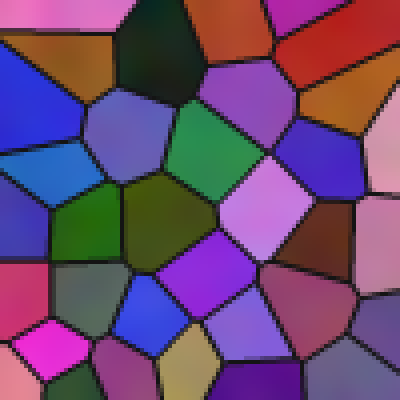
\includegraphics[width=6.6mm]{assets/drawn/diffusion-t0}};
    \draw[flow,draw=udsblue] ([xshift=0.6mm]u0.east) -- ([xshift=-0.6mm]u1.west);
    \node[way text] at (59,-41.6) {from noise alone, step by step: a new patch of any kind};
    % conditional: noise and a guide image
    \node[way name] at (2.4,-49.8) {conditional};
    \node[step image] (c0) at (27,-49.8) {
\includegraphics[width=6.6mm]{assets/drawn/diffusion-t1000}};
    \node[font=\small\bfseries,text=udsdark,inner sep=0pt] at (35.4,-49.8) {+};
    \node[step image] (c1) at (37.2,-49.8) {
\includegraphics[width=6.6mm]{assets/drawn/grain-map-blurred}};
    \draw[udsred,line width=0.6pt] (c1.south west) rectangle (c1.north east);
    \node[step image] (c2) at (49.4,-49.8) {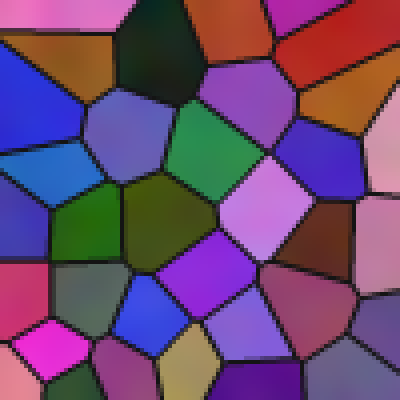
\includegraphics[width=6.6mm]{assets/drawn/diffusion-t0}};
    \draw[flow,draw=udsblue] ([xshift=0.6mm]c1.east) -- ([xshift=-0.6mm]c2.west);
    \node[way text] at (59,-49.8) {the U-Net also sees a \textcolor{udsred}{guide} at every step, here the VAE
      output};
  \end{tikzpicture}
  \note{\textbf{7:40--8:50}\par
    A diffusion model learns to undo noise.\par
    The forward process is fixed: each of 1000 steps scales the image down slightly and adds a little
      Gaussian noise $\epsilon$, with $\beta_t$ rising from 0.0001 to 0.02; after a few hundred steps only
      noise is left.\par
    Each step depends only on the one before, a Markov chain; the paper writes it as a Gaussian, its
      Eq.~12.\par
    The reverse process is learned: a network predicts the noise in an image at any step, and removing it
      step by step runs the process backwards.\par
    The idea is from Sohl-Dickstein and colleagues, 2015; DDPM, from Ho, Jain and Abbeel in 2020, made
      the images sharp.\par
    Once trained, it generates in two ways: from noise alone, any new patch; or with a guide image that
      the U-Net sees at every step, a patch that follows the guide.\par
    The paper's guide is the VAE's blurry output, so the diffusion model only restores detail; the next
      slide shows the training.}
\end{frame}

% ---------------------------------------------------- training a diffusion model
\begin{frame}[source={Ho et al.\ (2020), NeurIPS · Ronneberger et al.\ (2015), MICCAI}]
  {Training a diffusion model}
  \begin{tikzpicture}[x=1mm,y=1mm]
    \useasboundingbox (0,0) rectangle (144,-54);
    \begin{scope}[yshift=1mm]% content starts 4 mm below the title
    % a patch and a noise image, mixed in one go to a random step t
    \node[anchor=north west,inner sep=0pt] (x0) at (0,-1) {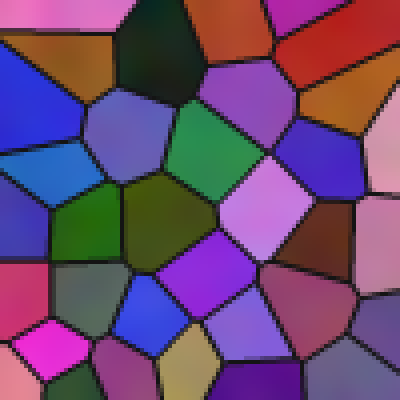
\includegraphics[width=12mm]{assets/drawn/diffusion-t0}};
    \node[anchor=north,small label,text=udsdark] at (6,-13.8) {patch $x_0$};
    \node[anchor=north west,inner sep=0pt] (eps) at (0,-21) {
\includegraphics[width=12mm]{assets/drawn/diffusion-noise}};
    \node[anchor=north,small label,text=udsdark] at (6,-33.8) {noise $\epsilon$};
    \node[draw=udsgreymid,fill=darktint,line width=0.5pt,inner sep=1.6mm,align=center,font=\footnotesize,
      text=udsdark] (mix) at (39,-7)
      {{\scriptsize\color{udsgrey}a random step $t$, in one go}\\[0.6mm]
       $x_t=\sqrt{\bar\alpha_t}\,x_0+\sqrt{1-\bar\alpha_t}\,\epsilon$};
    \draw[flow] (x0.east) -- (x0.east -| mix.west);
    \draw[flow] (12,-24) to[out=0,in=-90] (30,-12.6 |- mix.south);
    % the noised patch and its step go into the U-Net, which predicts the noise
    \node[anchor=north west,inner sep=0pt] (xt) at (66,-1) {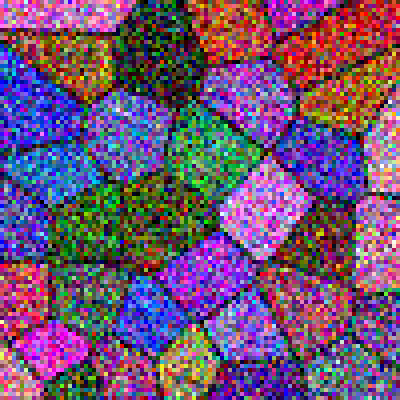
\includegraphics[width=12mm]{assets/drawn/diffusion-t150}};
    \node[anchor=north,small label,text=udsdark] at (72,-13.8) {$x_t$, here $t=150$};
    \draw[flow] (mix.east) -- (mix.east -| xt.west);
    \node[draw=udsblue,fill=bluetint,line width=0.5pt,minimum width=14mm,minimum height=9mm,font=\footnotesize,
      text=udsblue,inner sep=0pt] (unet) at (92,-7) {U-Net};
    \draw[flow] (xt.east |- unet.west) -- (unet.west);
    \node[anchor=north,small label,text=udsdark] (tin) at (92,-17.4) {step $t$};
    \draw[flow,line width=0.5pt] (tin.north) -- (unet.south);
    \node[anchor=west,font=\footnotesize,text=udsblue,inner sep=0pt] (pred) at (105.2,-7) {$\epsilon_\theta(x_t,t)$};
    \node[anchor=north,small label,text=udsblue] at ([yshift=-1.4mm]pred.south) {predicted noise};
    \draw[flow] (unet.east) -- (pred.west);
    % the loss: the predicted noise against the noise that was added
    \node[draw=udsred,fill=redtint,line width=0.5pt,inner sep=1.6mm,font=\footnotesize,text=udsdark] (loss)
      at (pred.center |- 0,-29) {$\|\epsilon-\epsilon_\theta(x_t,t)\|^2$};
    \draw[flow] ([yshift=-5.6mm]pred.south) -- (loss.north);
    \draw[flow,draw=udsred] (eps.east |- loss.west) -- (loss.west);
    \node[anchor=south,small label,text=udsred] at (56,-28.4) {the noise that was added is the target};
    \node[anchor=west,small label,text width=14mm] at ([xshift=1.6mm]loss.east) {loss: trains the U-Net};
    \end{scope}
    % repeated over many patches; the paper adds the VAE output as an input
    \fill[bluetint] (0,-40.4) rectangle (70,-53.6);
    \node[card text,anchor=west,text width=66mm] at (2,-47) {repeated over many patches, steps and noise
      images: one U-Net learns all 1000 steps};
    \fill[redtint] (74,-40.4) rectangle (144,-53.6);
    \node[card text,anchor=west,text width=66mm] at (76,-47) {Liao et al.: the U-Net also sees the VAE output,
      $\epsilon_\theta(x_t,t,x_V)$};
  \end{tikzpicture}
  \note{\textbf{8:50--10:00}\par
    A diffusion model is trained on one simple task: predict the noise in a noised image.\par
    Take a training patch $x_0$, draw a noise image $\epsilon$ and a random step $t$, and mix them in one
      go; $\bar\alpha_t$, the product of all $1-\beta_s$ up to step $t$, says how much of the patch is
      left.\par
    The network, a U-Net (Ronneberger and colleagues, 2015), gets the noised patch and the step and returns
      a noise image of the same size.\par
    The loss is the squared error between the added and the predicted noise; repeated over many patches,
      steps and noise images, one network learns every step.\par
    Knowing the noise is enough to step back: each reverse step subtracts a share of the predicted noise
      and adds a little fresh noise.\par
    The paper trains its diffusion model this way, with the VAE output $x_V$ as a third input, and
      compares the noise with the loss of section 3.}
\end{frame}

% --------------------------------------------------------- Pareto, NSGA-II
\begin{frame}[source={Pareto (1906), \emph{Manuale di economia politica} · Holland (1975), \emph{Adaptation in Natural and Artificial Systems} · Deb et al.\ (2002), IEEE Trans.\ Evol.\ Comput.\ 6, 182}]
  {Pareto fronts and NSGA-II}
  \begin{tikzpicture}[x=1mm,y=1mm]
    \useasboundingbox (0,0) rectangle (144,-54);
    \tikzset{panel frame/.style={draw=udsgreylight,line width=0.5pt,rounded corners=1mm},
      name part/.style={anchor=north,inner sep=0pt,font=\Large\bfseries,text=udsblue},
      name meaning/.style={anchor=north,small label,text=udsdark},
      front point/.style={circle,fill=udsblue,inner sep=0pt,minimum size=1.6mm},
      back point/.style={circle,fill=udsgreymid,inner sep=0pt,minimum size=1.6mm},
      point name/.style={inner sep=0pt,font=\scriptsize\bfseries,text=udsdark},
      ga row/.style={anchor=west,label text},
      ga icon/.style={font=\footnotesize,text=udsblue}}
    % the name, part by part, over the panel that explains each part
    \foreach \x/\l/\m in {22/NS/non-dominated sorting,72/GA/genetic algorithm,122/II/crowding distance} {
      \node[name part] at (\x,0) {\l};
      \node[name meaning] at (\x,-5.2) {\m};}
    \foreach \x in {0,50,100} \draw[panel frame] (\x,-9.2) rectangle ++(44,-38.4);
    % NS: A beats B in both goals; nobody beats A, C or D in both, so they form front 1
    \begin{scope}[shift={(5,-43.6)}]
      \draw[udsgreymid,line width=0.5pt,-{Stealth[length=1.4mm,width=1mm]}] (0,0) -- (38,0);
      \draw[udsgreymid,line width=0.5pt,-{Stealth[length=1.4mm,width=1mm]}] (0,0) -- (0,30.4);
      \node[anchor=north east,small label] at (38,-0.6) {goal 1};
      \node[anchor=south east,small label,rotate=90] at (-0.6,30.4) {goal 2};
      \begin{scope}[x=36mm,y=29mm]
        \fill[redtint] (0,0) rectangle (0.8,0.8);
        \node[anchor=south west,small label,text=udsred] at (0.04,0.05) {A beats B in both};
        \draw[udsgreymid,line width=0.6pt,dash pattern=on 1.4pt off 1pt]
          (0.35,0.75) -- (0.35,0.6) -- (0.6,0.6) -- (0.6,0.4) -- (0.7,0.4);
        \draw[udsblue,line width=0.8pt] (0.5,0.95) -- (0.5,0.8) -- (0.8,0.8) -- (0.8,0.5) -- (0.95,0.5);
        \foreach \u/\v in {0.5/0.95,0.8/0.8,0.95/0.5} \node[front point] at (\u,\v) {};
        \foreach \u/\v in {0.35/0.75,0.6/0.6,0.7/0.4} \node[back point] at (\u,\v) {};
        \foreach \n/\u/\v/\dx/\dy/\a in {A/0.8/0.8/0.9/0.9/south west,B/0.6/0.6/0.9/0.9/south west,
            C/0.95/0.5/0/1.2/south,D/0.5/0.95/-1.2/0/east}
          \node[point name,anchor=\a] at ([shift={(\dx mm,\dy mm)}]\u,\v) {\n};
        \node[anchor=west,small label,text=udsblue] at (0.56,0.97) {front 1};
        \node[anchor=north west,small label,text=udsgreymid] at (0.36,0.57) {front 2};
      \end{scope}
    \end{scope}
    % GA: one generation, top to bottom, and round again
    \foreach \y/\icon/\t in {-14.4/\faUsers/population,-22.4/\faBalanceScale/score both goals,
        -30.4/\faFilter/{keep the best: by front,\\ then by crowding},-38.4/\faRandom/{cross over, mutate}} {
      \node[ga icon] at (57.6,\y) {\icon};
      \node[ga row] at (62.4,\y) {\t};}
    \foreach \y in {-14.4,-22.4,-30.4} \draw[flow,draw=udsblue,line width=0.5pt] (57.6,\y-2.4) -- (57.6,\y-5.6);
    \draw[flow,draw=udsblue,line width=0.5pt] (55,-38.4) -- (52.6,-38.4) -- (52.6,-14.4) -- (55,-14.4);
    \node[anchor=north,small label,text=udsdark] at (71.5,-42.2) {repeat for hundreds of generations};
    % the two rules of "keep the best" come from the panels beside it
    \draw[flow,draw=udsblue] (44.6,-30.4) -- (49.4,-30.4);
    \draw[flow,draw=udsblue] (99.4,-30.4) -- (94.6,-30.4);
    % II: on a crowded front, near-copies are dropped and points with room around them kept
    \begin{scope}[shift={(105,-43.6)}]
      \draw[udsgreymid,line width=0.5pt,-{Stealth[length=1.4mm,width=1mm]}] (0,0) -- (38,0);
      \draw[udsgreymid,line width=0.5pt,-{Stealth[length=1.4mm,width=1mm]}] (0,0) -- (0,30.4);
      \node[anchor=north east,small label] at (38,-0.6) {goal 1};
      \node[anchor=south east,small label,rotate=90] at (-0.6,30.4) {goal 2};
      \begin{scope}[x=36mm,y=29mm]
        \draw[testgreen,line width=0.6pt,dash pattern=on 1.2pt off 0.8pt] (0.12,0.62) rectangle (0.76,0.95);
        \draw[udsblue,line width=0.8pt] (0.12,0.95) -- (0.12,0.85) -- (0.45,0.85) -- (0.45,0.62) -- (0.76,0.62)
          -- (0.76,0.6) -- (0.8,0.6) -- (0.8,0.58) -- (0.84,0.58) -- (0.84,0.3) -- (0.95,0.3);
        \foreach \u/\v in {0.12/0.95,0.45/0.85,0.76/0.62,0.8/0.6,0.84/0.58,0.95/0.3} \node[front point] at (\u,\v) {};
        \node[text=udsred,font=\footnotesize\bfseries,inner sep=0pt] at (0.8,0.6) {\faTimes};
        \node[anchor=south west,small label,text=testgreen] at (0.17,0.965) {room around it: kept};
        \node[anchor=north east,small label,text=udsred,align=right] at (0.81,0.53) {near-copy:\\ dropped};
      \end{scope}
    \end{scope}
  \end{tikzpicture}
  \note{\textbf{10:00--11:20}\par
    With two goals that fight each other, such as strength and ductility, there is rarely one best
      answer, only a menu of trade-offs.\par
    NSGA-II, from Deb and colleagues in 2002, searches for that menu, and its name says how.\par
    GA, a genetic algorithm (Holland, 1975): a population of candidates evolves over generations; each is
      scored on both goals, the best become parents, and children mix their parents' parts (crossover)
      with small random changes (mutation).\par
    NS, non-dominated sorting: A beats B because it is better in both goals; nobody beats A, C or D in
      both, so they form front 1, the Pareto front, after Vilfredo Pareto, 1906; without front 1, the
      unbeaten rest form front 2, and the best are taken front by front.\par
    II, crowding distance: when a front has more candidates than places, near-copies are dropped and
      candidates with room around them are kept, so the population spreads along the whole front.\par
    Section 3 shows how the paper runs this search.}
\end{frame}
